\chapter{Introducción}
\noindent En la introducción se situará el contexto del trabajo realizado, identificando claramente el problema que se plantea y soluciones para el mismo que se hayan propuesto previamente. 

No hay máximo ni mínimo en cuanto a la extensión de la memoria del TFM, pero se debe buscar un equilibrio entre síntesis y completitud. 50 a 80 páginas más anexos suele ser suficiente.

\noindent La estructura de la memoria del TFM deberá reflejar, al menos, los siguientes contenidos:
\begin{itemize}
	\item Portada con título del TFM, nombres del autor y tutores, logotipo de la UPV y el Departamento de Ingeniería Electrónica, fecha (mes, año) y curso académico en el que realizó la defensa del TFM.
	\item  Índice de contenidos.
	\item  Introducción, en la que se situará el contexto del trabajo realizado, identificando claramente el problema que se plantea y soluciones para el mismo que se hayan propuesto previamente.
	\item  Descripción de la solución o las soluciones estudiadas.
	\item  Presentación de resultados tanto analíticos como de simulación y experimentales.
	\item  Conclusiones, en las que se hará un balance crítico de los resultados alcanzados.
	\item  Propuesta de actividades a desarrollar en el futuro, incluyendo, si fuera el caso, la línea de trabajo sobre la que se realizaría una futura tesis doctoral.
	\item  Referencias.
	\item  Anexos (si procede). En este apartado se pueden añadir esquemas electrónicos, detalles de cálculos largos, desarrollos matemáticos largos, hojas de datos que se considere imprescindibles, etc.
\end{itemize}


\chapter{Formato de la Memoria}
\section{Idioma}
\noindent La memoria se podrá escribir en castellano, valenciano o inglés.
\section{Tipo de letra y tamaño de página}
\noindent La memoria podrá estar realizada en cualquier formato que se pueda convertir a PDF (Word, \TeX,...) y se usará letra Book Antiqua, Times New Roman, Calibri o Arial de tamaño 11 puntos. El tamaño de página será A4 con márgenes superior e inferior 2,5 cm, márgenes izquierdo y derecho 3 cm.
\section{Estructura}
\subsection{Párrafos}
\noindent La memoria se escribirá en párrafos justificados a izquierda y derecha. Se usará un interlineado sencillo con una separación entre párrafos mínima de 6 puntos.
\subsection{Capítulos, Secciones y Subsecciones}
\noindent Los capítulos irán numerados y se dividirán en secciones y subsecciones con la numeración correspondiente.  
\section{Figuras, tablas y ecuaciones}
\noindent Las tablas y las figuras tendrán su correspondiente numeración en el pie de las mismas, que dará una breve descripción y citará a la referencia de la que procede, si es el caso. Las ecuaciones también irán numeradas. La numeración puede dar cuenta del capítulo en que se encuentra la tabla, figura o ecuación, si el alto número así lo aconseja. Las figuras pueden contener subfiguras, por ejemplo la Figura~\mbox{\ref{fig:subfigs}(a)} y \mbox{\ref{fig:subfigs}(b)}. La Figura~\ref{fig:PLL2} es otro ejemplo.

Las Tablas~\ref{tab:ejemplo} y \ref{tab:tablagris2} son ejemplos de tabla.

\begin{figure}
	\centering
	\includegraphics[page=6,trim=3.5cm 10.75cm 3.5cm 2.5cm 0,clip]{Plantilla_Memoria_TFM_PDF-2018.pdf}
	\caption{Ejemplo de figura con dos subfiguras. (a) descripción de la figura superior. (b) descripción de la figura
		inferior. }
	\label{fig:subfigs}
\end{figure}
\begin{figure}
	\centering
	\resizebox{\textwidth}{!}{\begin{tikzpicture}[ultra thick,black,opacity=1]
			\tikzset{bloque/.style={draw=black, rectangle,draw=blue, fill=lightgray!20, rounded corners,minimum width=2cm,minimum height=1cm,ultra thick}}
			\node[bloque] at (0,0) (PC){\shortstack{Phase\\comparator}};
			\node[bloque] at (3,0) (LF){\shortstack{Loop\\filter}};
			\node[bloque] at (6,0) (VCO){\shortstack{VCO}};
			\node[circle,fill=black,draw=black,inner sep=0.5mm] at ($(VCO.east)+(0.5cm,0)$) (nodo){};
			\draw[latex-] (PC.west) -- +(-1,0) node[pos=1,anchor=east](){$V_i$};
			\draw[-latex] (VCO.east) -- +(1,0) node[pos=1,anchor=west](){$V_o$};
			\draw[-latex] (nodo) -- +(0,-1)  -| (PC);
			\draw[-latex] (PC) -- (LF);
			\draw[-latex] (LF) -- (VCO);
	\end{tikzpicture}}
	\caption{Ejemplo de figura}
	\label{fig:PLL2}
\end{figure}

\begin{table}[]
	\centering
	\begin{tabular}{@{} *5l @{}}    \toprule
		\emph{name} & \emph{foo} &&&  \\\midrule
		Models    & A  & B  & C  & D  \\ 
		Model $X$ & X1 & X2 & X3 & X4\\ 
		Model $Y$ & Y1 & Y2 & Y3 & Y4\\\bottomrule
		\hline
	\end{tabular}
	\caption{Tabla ejemplo}
	\label{tab:ejemplo}
\end{table}

\begin{table}[]
	\centering
	\begin{tikzpicture}
		\node[inner sep=0pt,outer sep=0pt] (tbl) {
			\begin{tabularx}{.75\textwidth}{ p{0.15 \textwidth}  p{0.10 \textwidth} p{0.10 \textwidth} p{0.10 \textwidth} p{0.15 \textwidth}  }
				\toprule
				& Small  &  Medium &  Large & Shape fraction \\
				\midrule
				Compact    & 10\% &  44\% & 7\% & 61\% \\ 
				Flat       & 4\%  &  10\% & 4\% & 18\% \\ 
				Elongated  & 5\%  &  12\% & 4\% & 21\% \\ 
				\midrule 
				Size fraction  & 19\% & 66\% & 15\% & 100\% \\
				\bottomrule
		\end{tabularx}};
		\begin{pgfonlayer}{background}
			\draw[top color=lightgray,bottom color=lightgray!10!white,
			draw=none] ($(tbl.north west)+(0,0)$)
			rectangle ($(tbl.north east)+(0,-1.9em)$);
			\draw[fill=white,draw=none] ($(tbl.south west)
			+(0,0)$) rectangle ($(tbl.north east)+(0,-1.9em)$);
		\end{pgfonlayer}
	\end{tikzpicture}
	\caption{Otra tabla}
	\label{tab:tablagris2}
\end{table}


Ejemplos de ecuaciones (\ref{eq:muise1}, \ref{eq:muise2} y \ref{eq:muise3}):
\begin{equation}
	\label{eq:muise1}
	\textrm{PF}=\frac{I_{1\_\textrm{RMS}}}{I_{\textrm{RMS}}}{\cdot}\cos\varphi_1
\end{equation}

\begin{equation}
	\label{eq:muise2}
	(1+x)^n=1+\frac{n x}{1!}+\frac{n (n-1)x^2}{2!}+\ldots
\end{equation}

\begin{align}
	\mathbb{X}[z]&=\sum_{n=0}^{N-1}x[n]{\cdot}z^{-n}
	=\sum_{n=0}^{\infty} a^{-n}{\cdot}z^{-n}=\nonumber\\
	\label{eq:muise3}
	&=\frac{1}{1-(a{\cdot}z)^{-1}}=\frac{z}{z{-}a^{-1}}
\end{align}

\section{Referencias bibliográficas}

\noindent Se debe incluir las referencias bibliográficas o de internet de las fuentes consultadas y/o
utilizadas en la memoria. Estas referencias deberán ser correctamente citadas en el texto, dando
siempre el debido reconocimiento a las fuentes de información. Se pueden listar en el apartado
de referencias con diferentes estilos.
Por ejemplo, numéricamente entre corchetes como se muestra en la bibliografía.

Citando una referencia \cite{Smith1997}, otra \cite{Orfanidis1996} y otra \cite{Wyndrum1965}. Y otra más \cite{Dai2010}.

\section{Lista de siglas empleadas}

Para que las siglas empleadas aparezcan en el listado de siglas, al principio del documento, hay que definirlas en ``siglas.tex'' y también usarlas en el documento con el comando \verb+\gls+: \gls{utc}, \gls{lna} y \gls{adt} se están usando de esa manera.